%%%%%%%%%%%%%%%%%%%%%%%%%%%%%%%%%%%%%%%%%%%%%%%%%%%%%%%%%%%%%%%

% Set up document

\documentclass{beamer}
\usecolortheme{whale}
\setbeamersize{text margin left=5mm,text margin right=5mm}

% Used to create a section slide between section
\AtBeginSection[]{
  \begin{frame}
  \vfill
  \centering
  \begin{beamercolorbox}[sep=8pt,center,shadow=true,rounded=true]{title}
    \usebeamerfont{title}\insertsectionhead\par%
  \end{beamercolorbox}
  \vfill
  \end{frame}
}

% Remove default navigation symbols and add just  page number
\setbeamertemplate{navigation symbols}{} % Clear default navigation
\addtobeamertemplate{navigation symbols}{}{%
    \usebeamerfont{footline}%
    \usebeamercolor[fg]{footline}%
    \hspace{1em}%
    \insertframenumber/\inserttotalframenumber
}


%%%%%%%%%%%%%%%%%%%%%%%%%%%%%%%%%%%%%%%%%%%%%%%%%%%%%%%%%%%%%%%

% Title page

\title{Stroke Audit Machine Learning (SAMueL)}
\subtitle{Learnings from explainable machine learning}


\author{Kerry Pearn\inst{1}, Michael Allen\inst{1,3}, Anna Laws\inst{1}, Richard Everson\inst{3}, Martin James\inst{1,2} }
\institute{\inst{1}University of Exeter Medical School \inst{2}Royal Devon University Healthcare NHS Foundation Trust \inst{3}University of Exeter Institute of Data Science and Artificial Intelligence}

%\institute{Overleaf}
\date{January 2023}


\begin{document}

%\frame{\titlepage}

\begin{frame}
\titlepage


\end{frame}


%%%%%%%%%%%%%%%%%%%%%%%%%%%%%%%%%%%%%%%%%%%%%%%%%%%%%%%%%%%%%%%

\begin{frame}
\frametitle{Machine learning overview}
\begin{center}
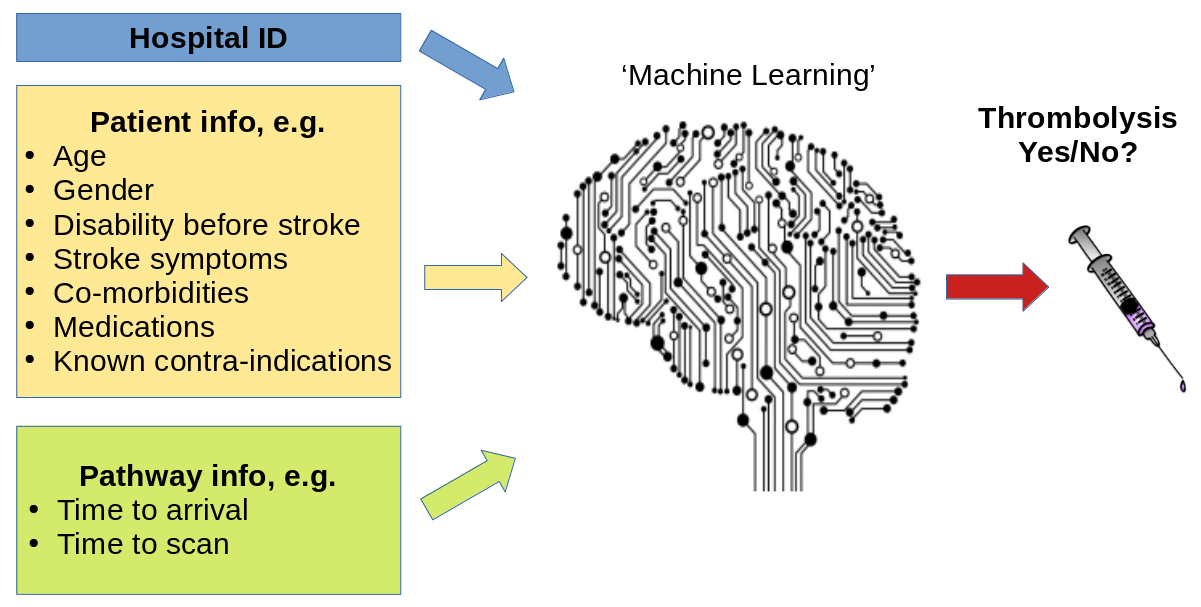
\includegraphics[width=0.85\textwidth]{./images/ml_model_high_level}
\end{center}

\small
Machine learning (and nearly all \emph{artificial intelligence}) is based on the simple principle of recognising similarity to what has been seen before.
\vspace{3mm}

We accessed 240,000 emergency stroke admissions in England and Wales over three years. Our machine learning models use XGBoost classification, and are based on all patients who arrive within 4 hours of known stroke onset. 
\end{frame}

%%%%%%%%%%%%%%%%%%%%%%%%%%%%%%%%%%%%%%%%%%%%%%%%%%%%%%%%%%%%%%%

\begin{frame}{Model accuracy, and simplification}

A model with all available 84 features had an ROC AUC of 0.922. A model with 10 features had an ROC AUC of 0.919.

\begin{center}
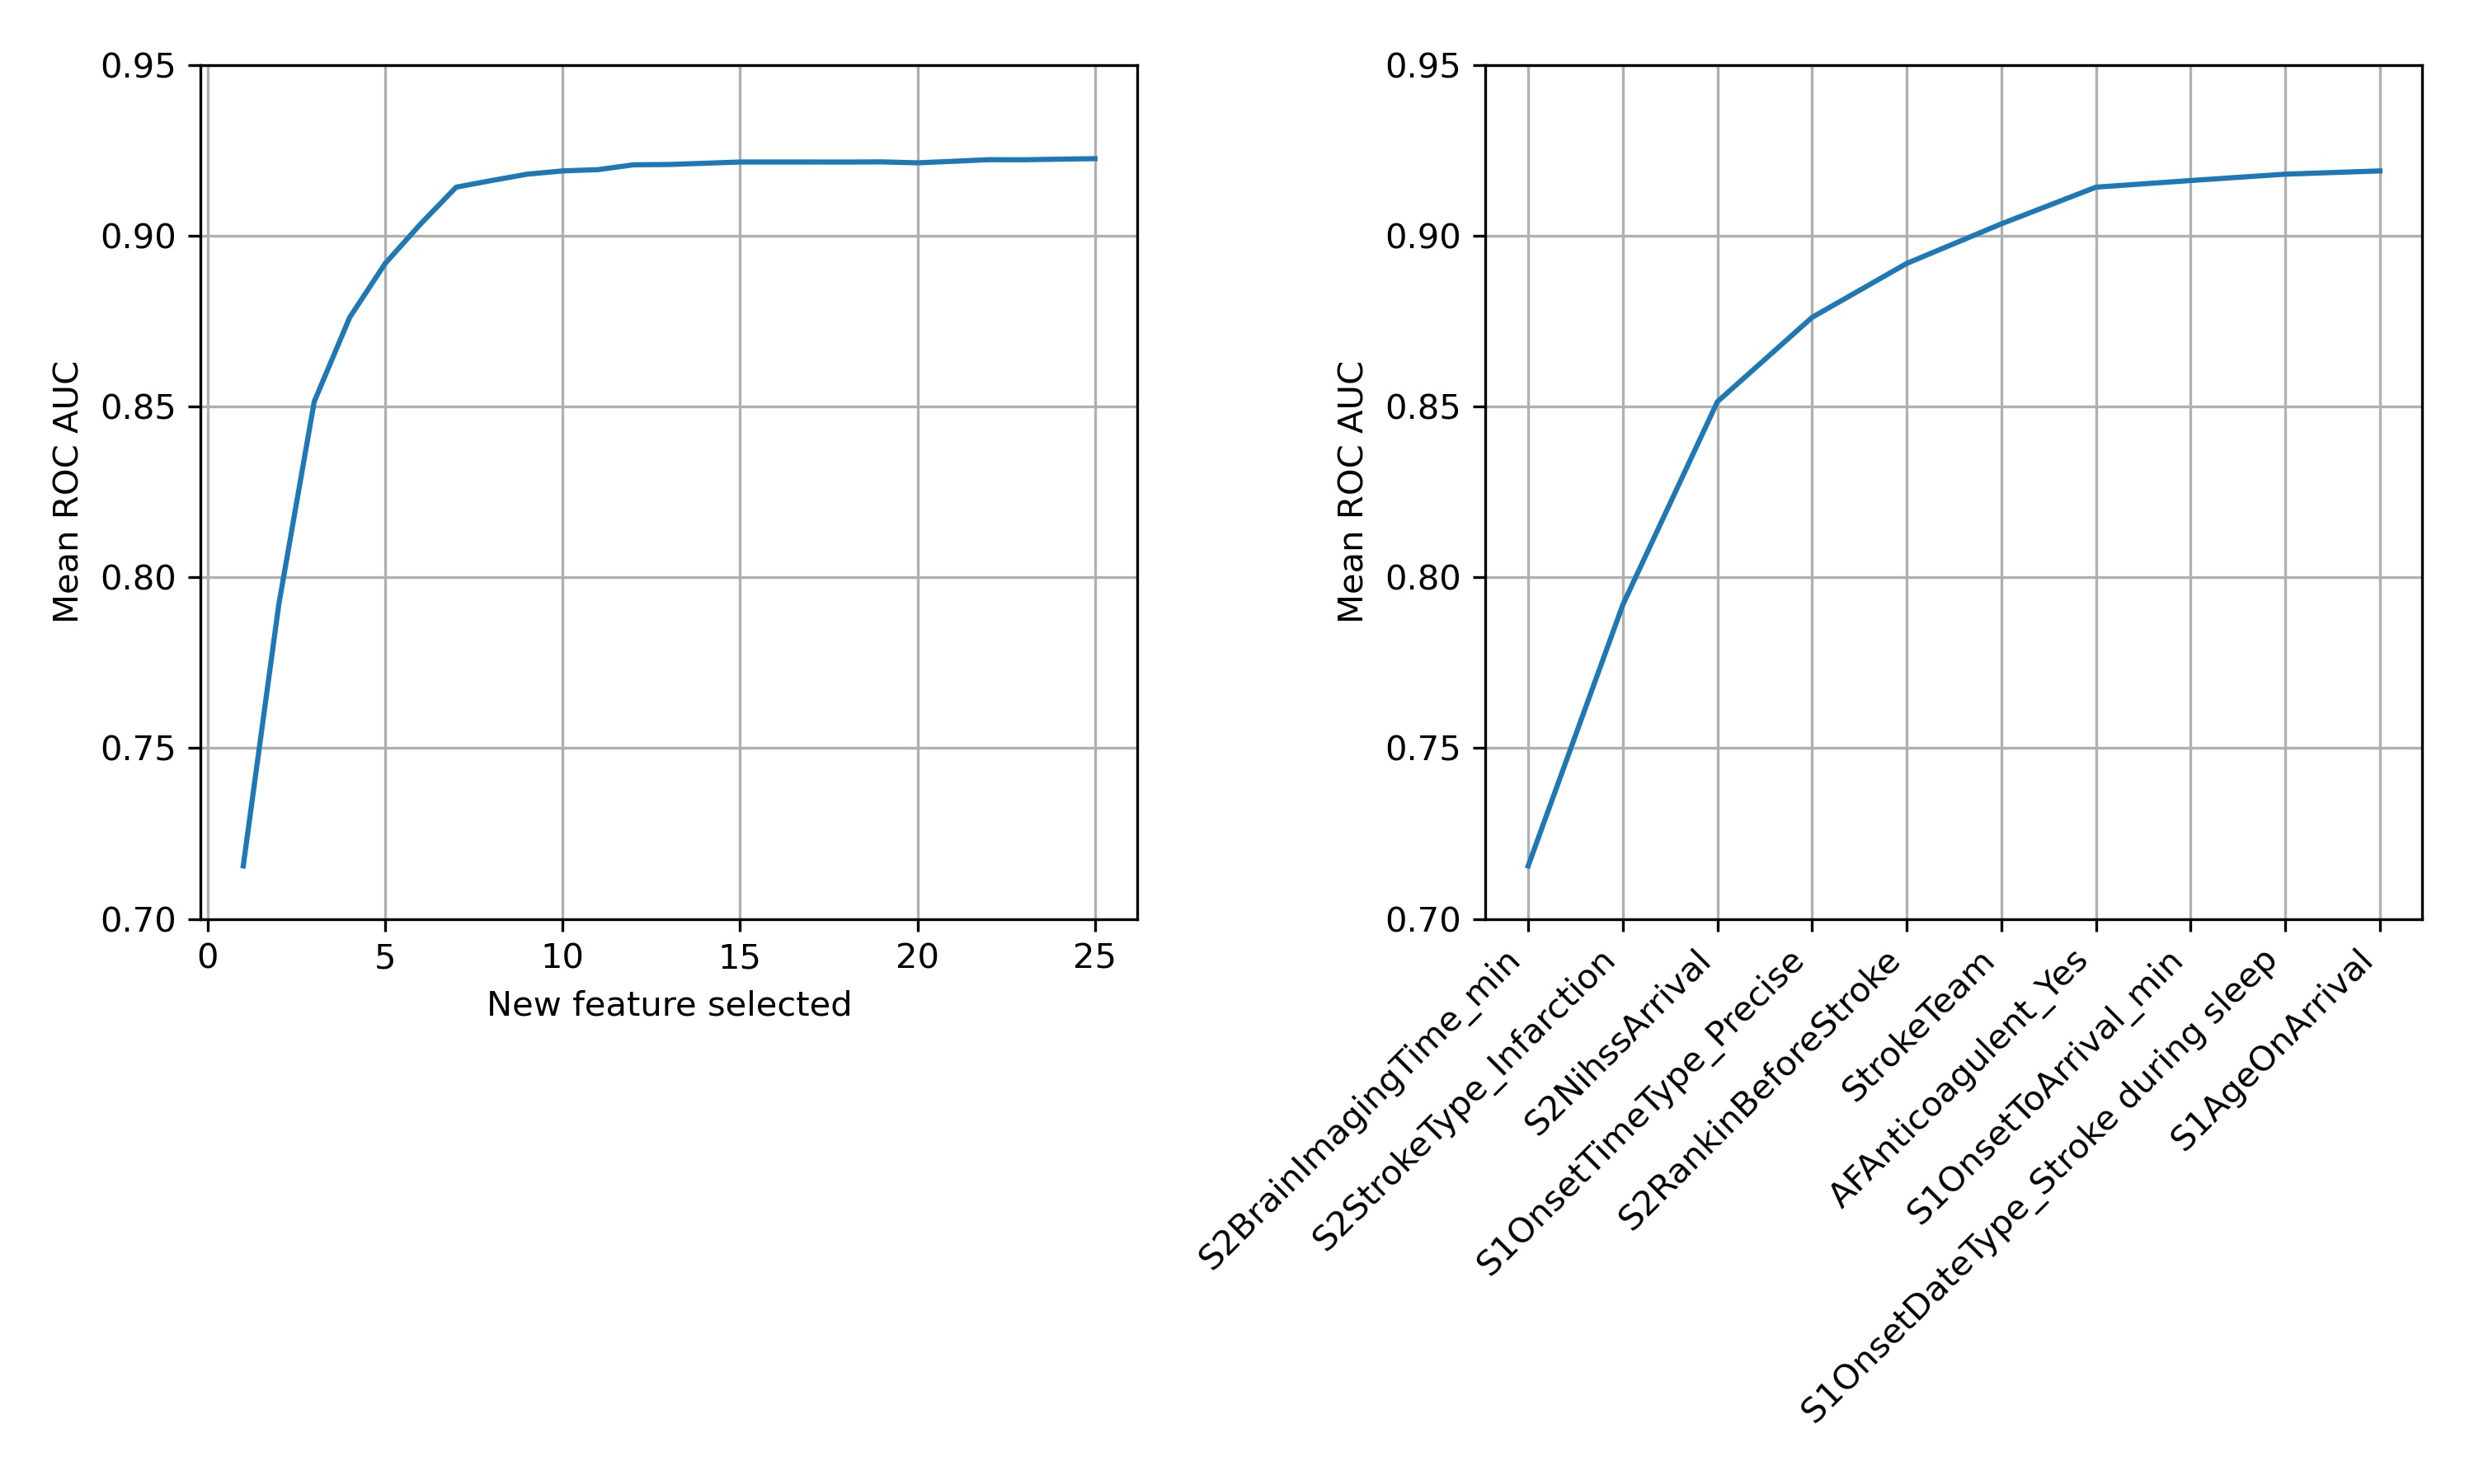
\includegraphics[width=1.0\textwidth]{./images/01_feature_selection.jpg}
\end{center}

\end{frame}


%%%%%%%%%%%%%%%%%%%%%%%%%%%%%%%%%%%%%%%%%%%%%%%%%%%%%%%%%%%%%%%

\begin{frame}{What do the most thrombolysable patients look like?}

For each hospital we identify the patient with the highest probability of receiving thrombolysis.

\begin{center}
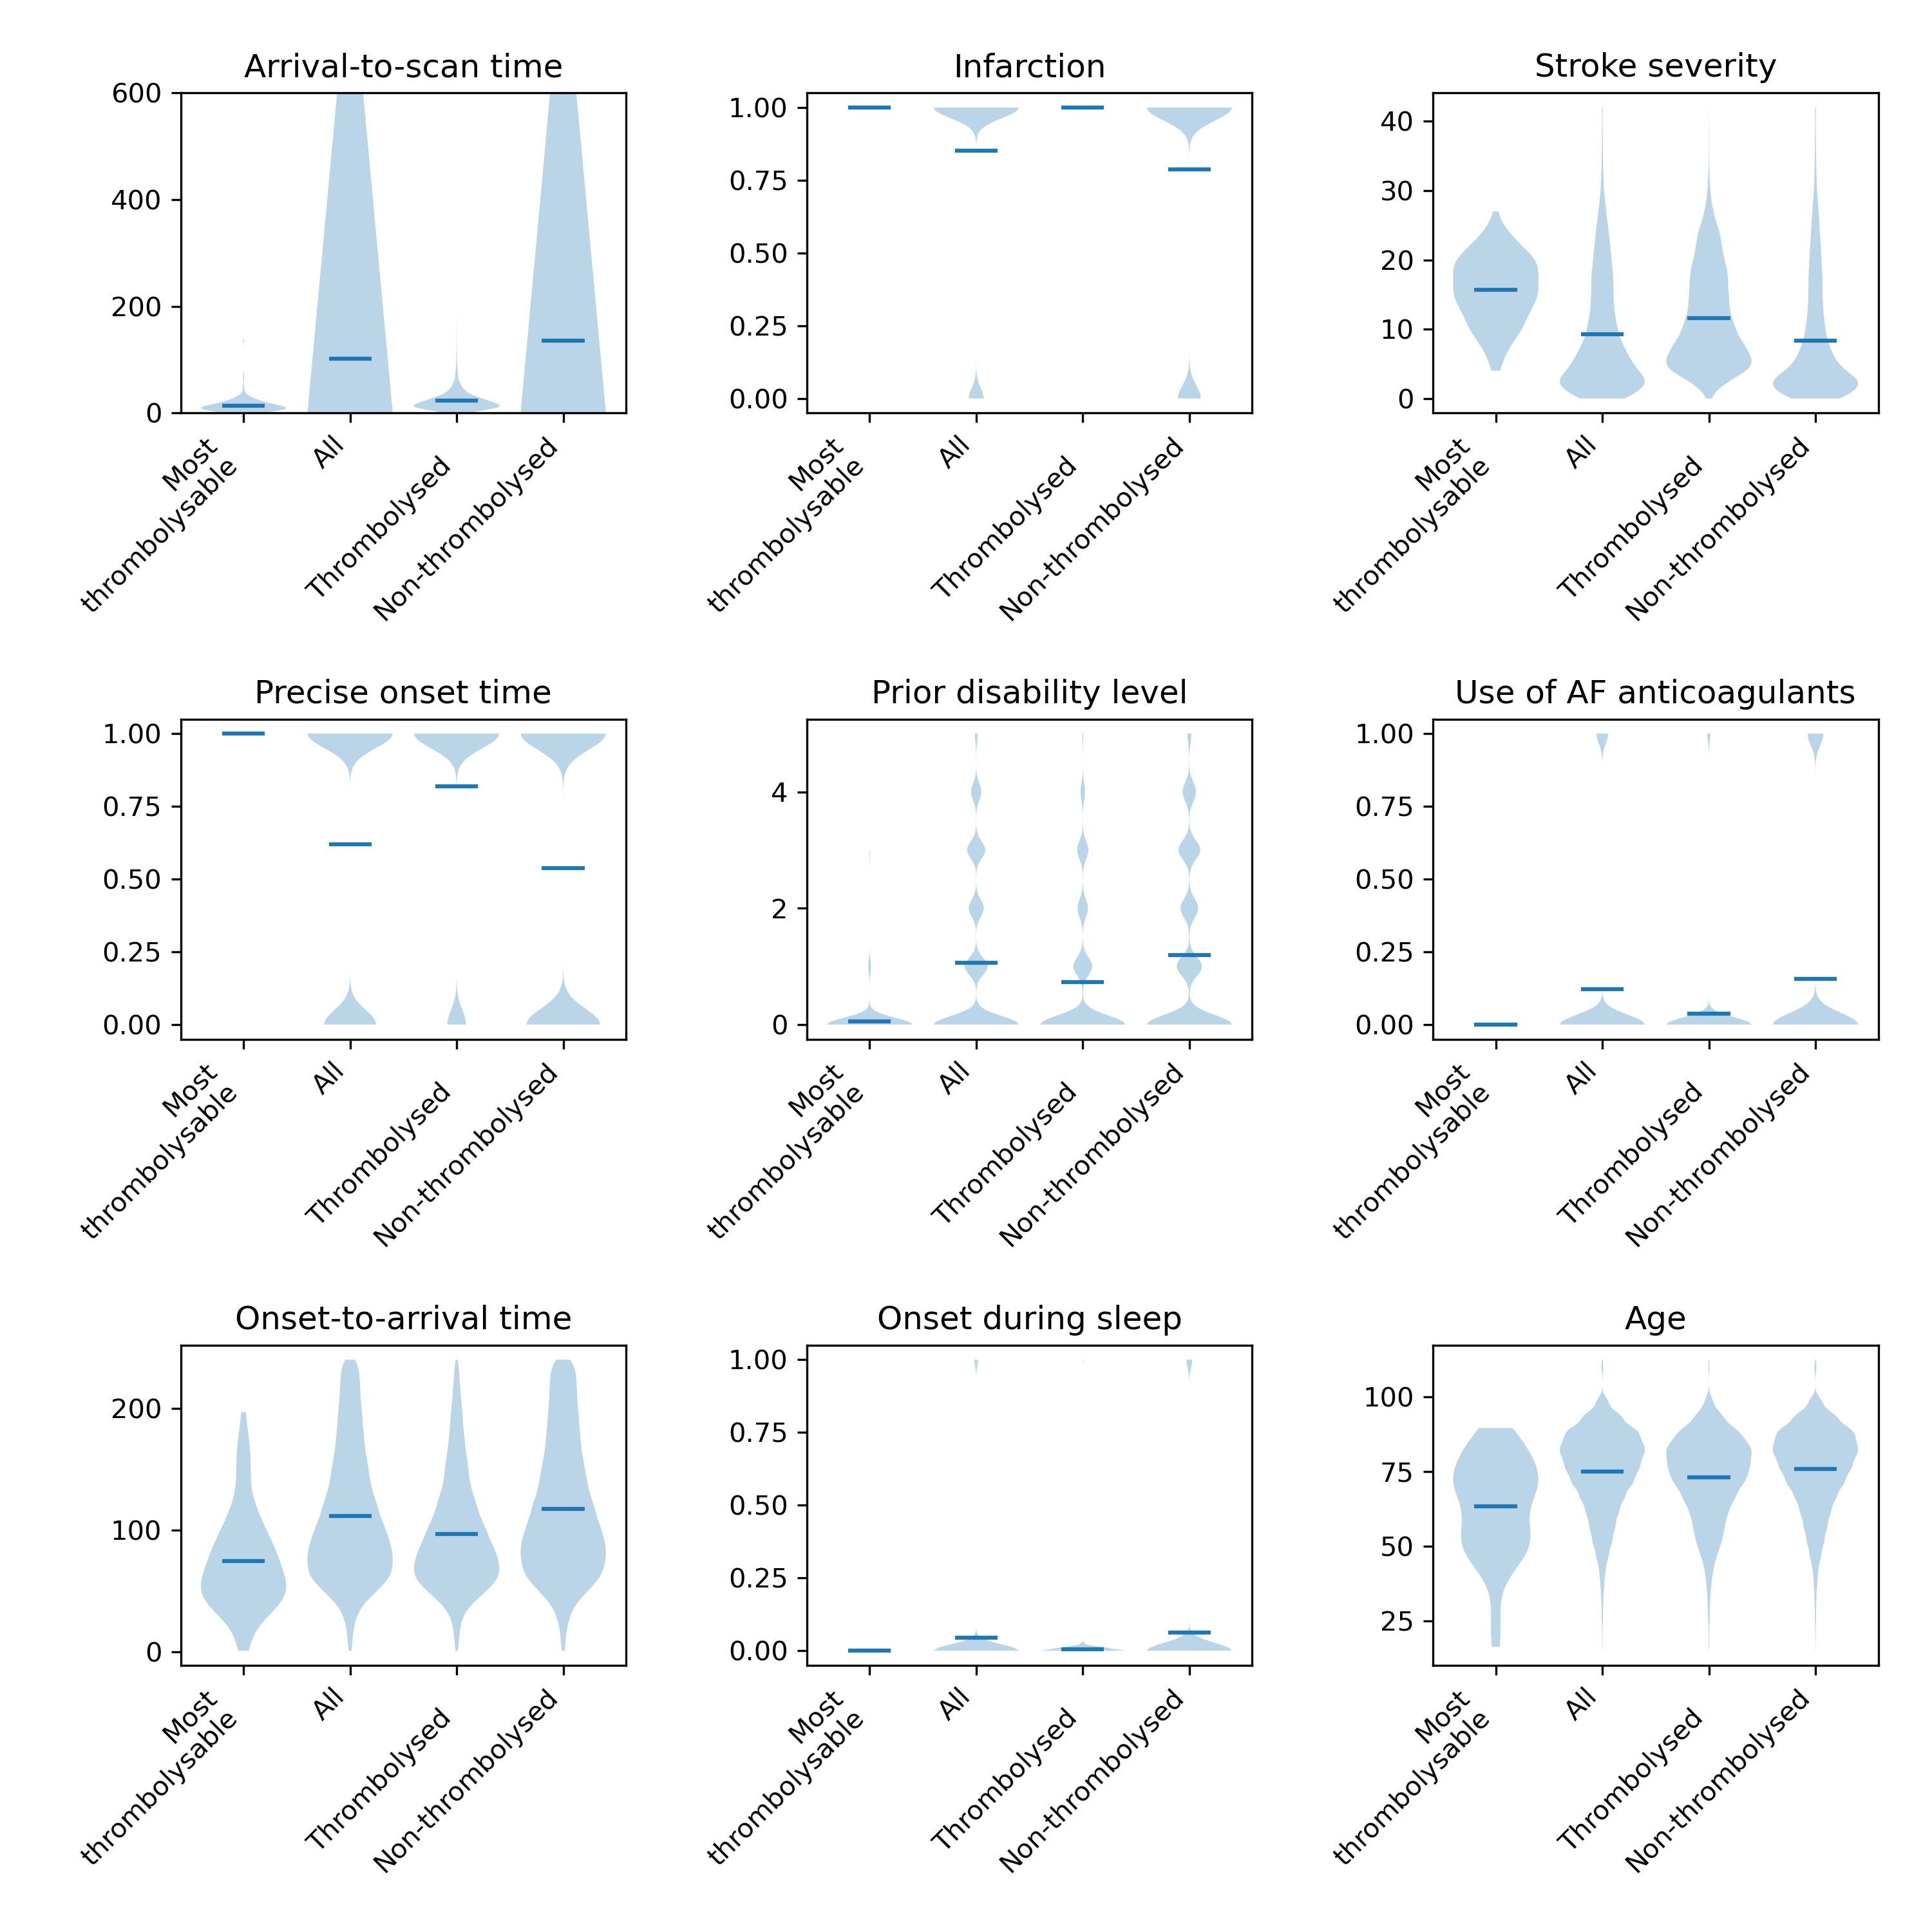
\includegraphics[width=0.6\textwidth]{./images/02a_most_thrombolsyable_violin.jpg}
\end{center}

\end{frame}





%%%%%%%%%%%%%%%%%%%%%%%%%%%%%%%%%%%%%%%%%%%%%%%%%%%%%%%%%%%%%%%

\begin{frame}
\frametitle{Explaining model predictions with SHAP values}

SHAP values show the influence of features (even for \emph{`black box'} models).

\begin{center}
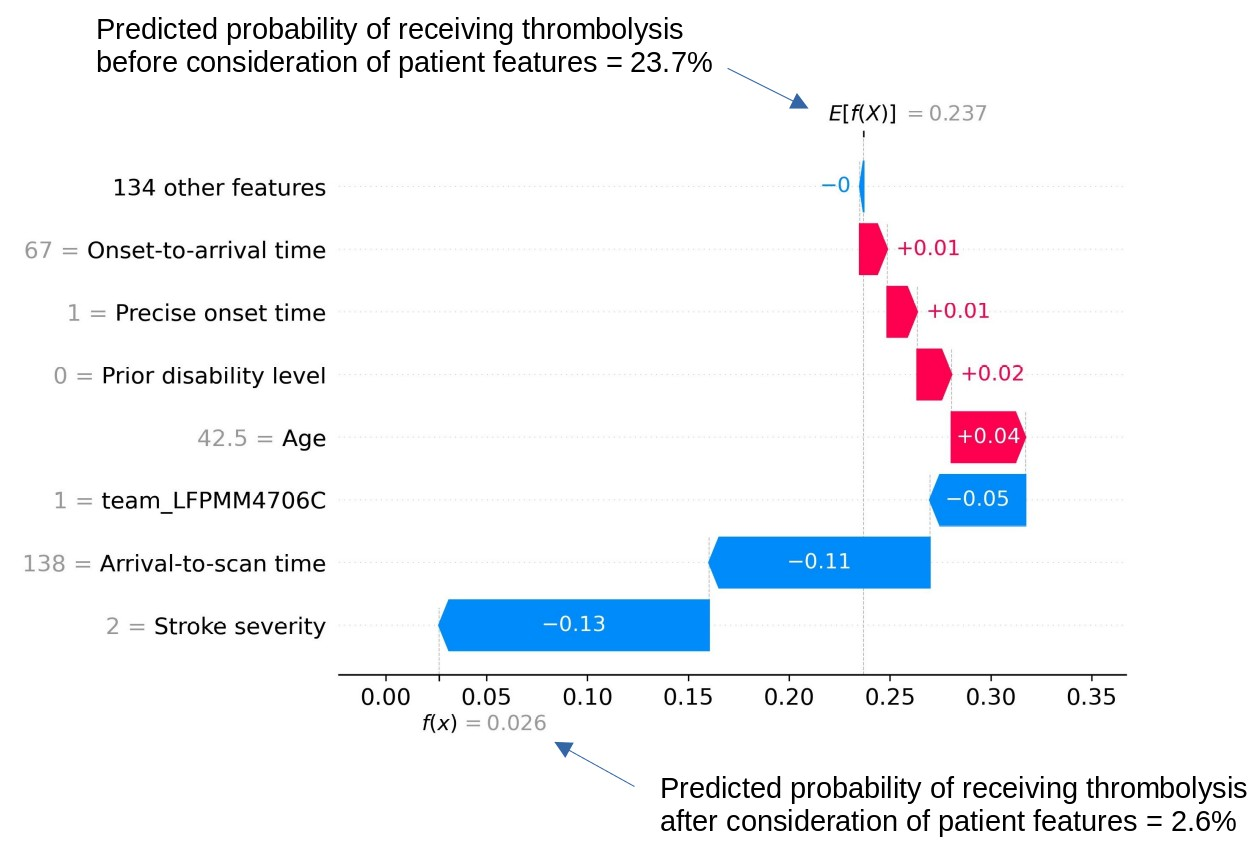
\includegraphics[width=0.90\textwidth]{./images/waterfall.jpg}
\end{center}
\end{frame}


%%%%%%%%%%%%%%%%%%%%%%%%%%%%%%%%%%%%%%%%%%%%%%%%%%%%%%%%%%%%%%%

\begin{frame}
\frametitle{What drives use of thrombolysis across all hospitals?}

\footnotesize{Note: SHAP values here are \emph{log odds}. Each step-change in value of \textpm 1 changes the chances of receiving thrombolysis about 3-fold. (Plots are in order of feature importance.)}

\begin{center}
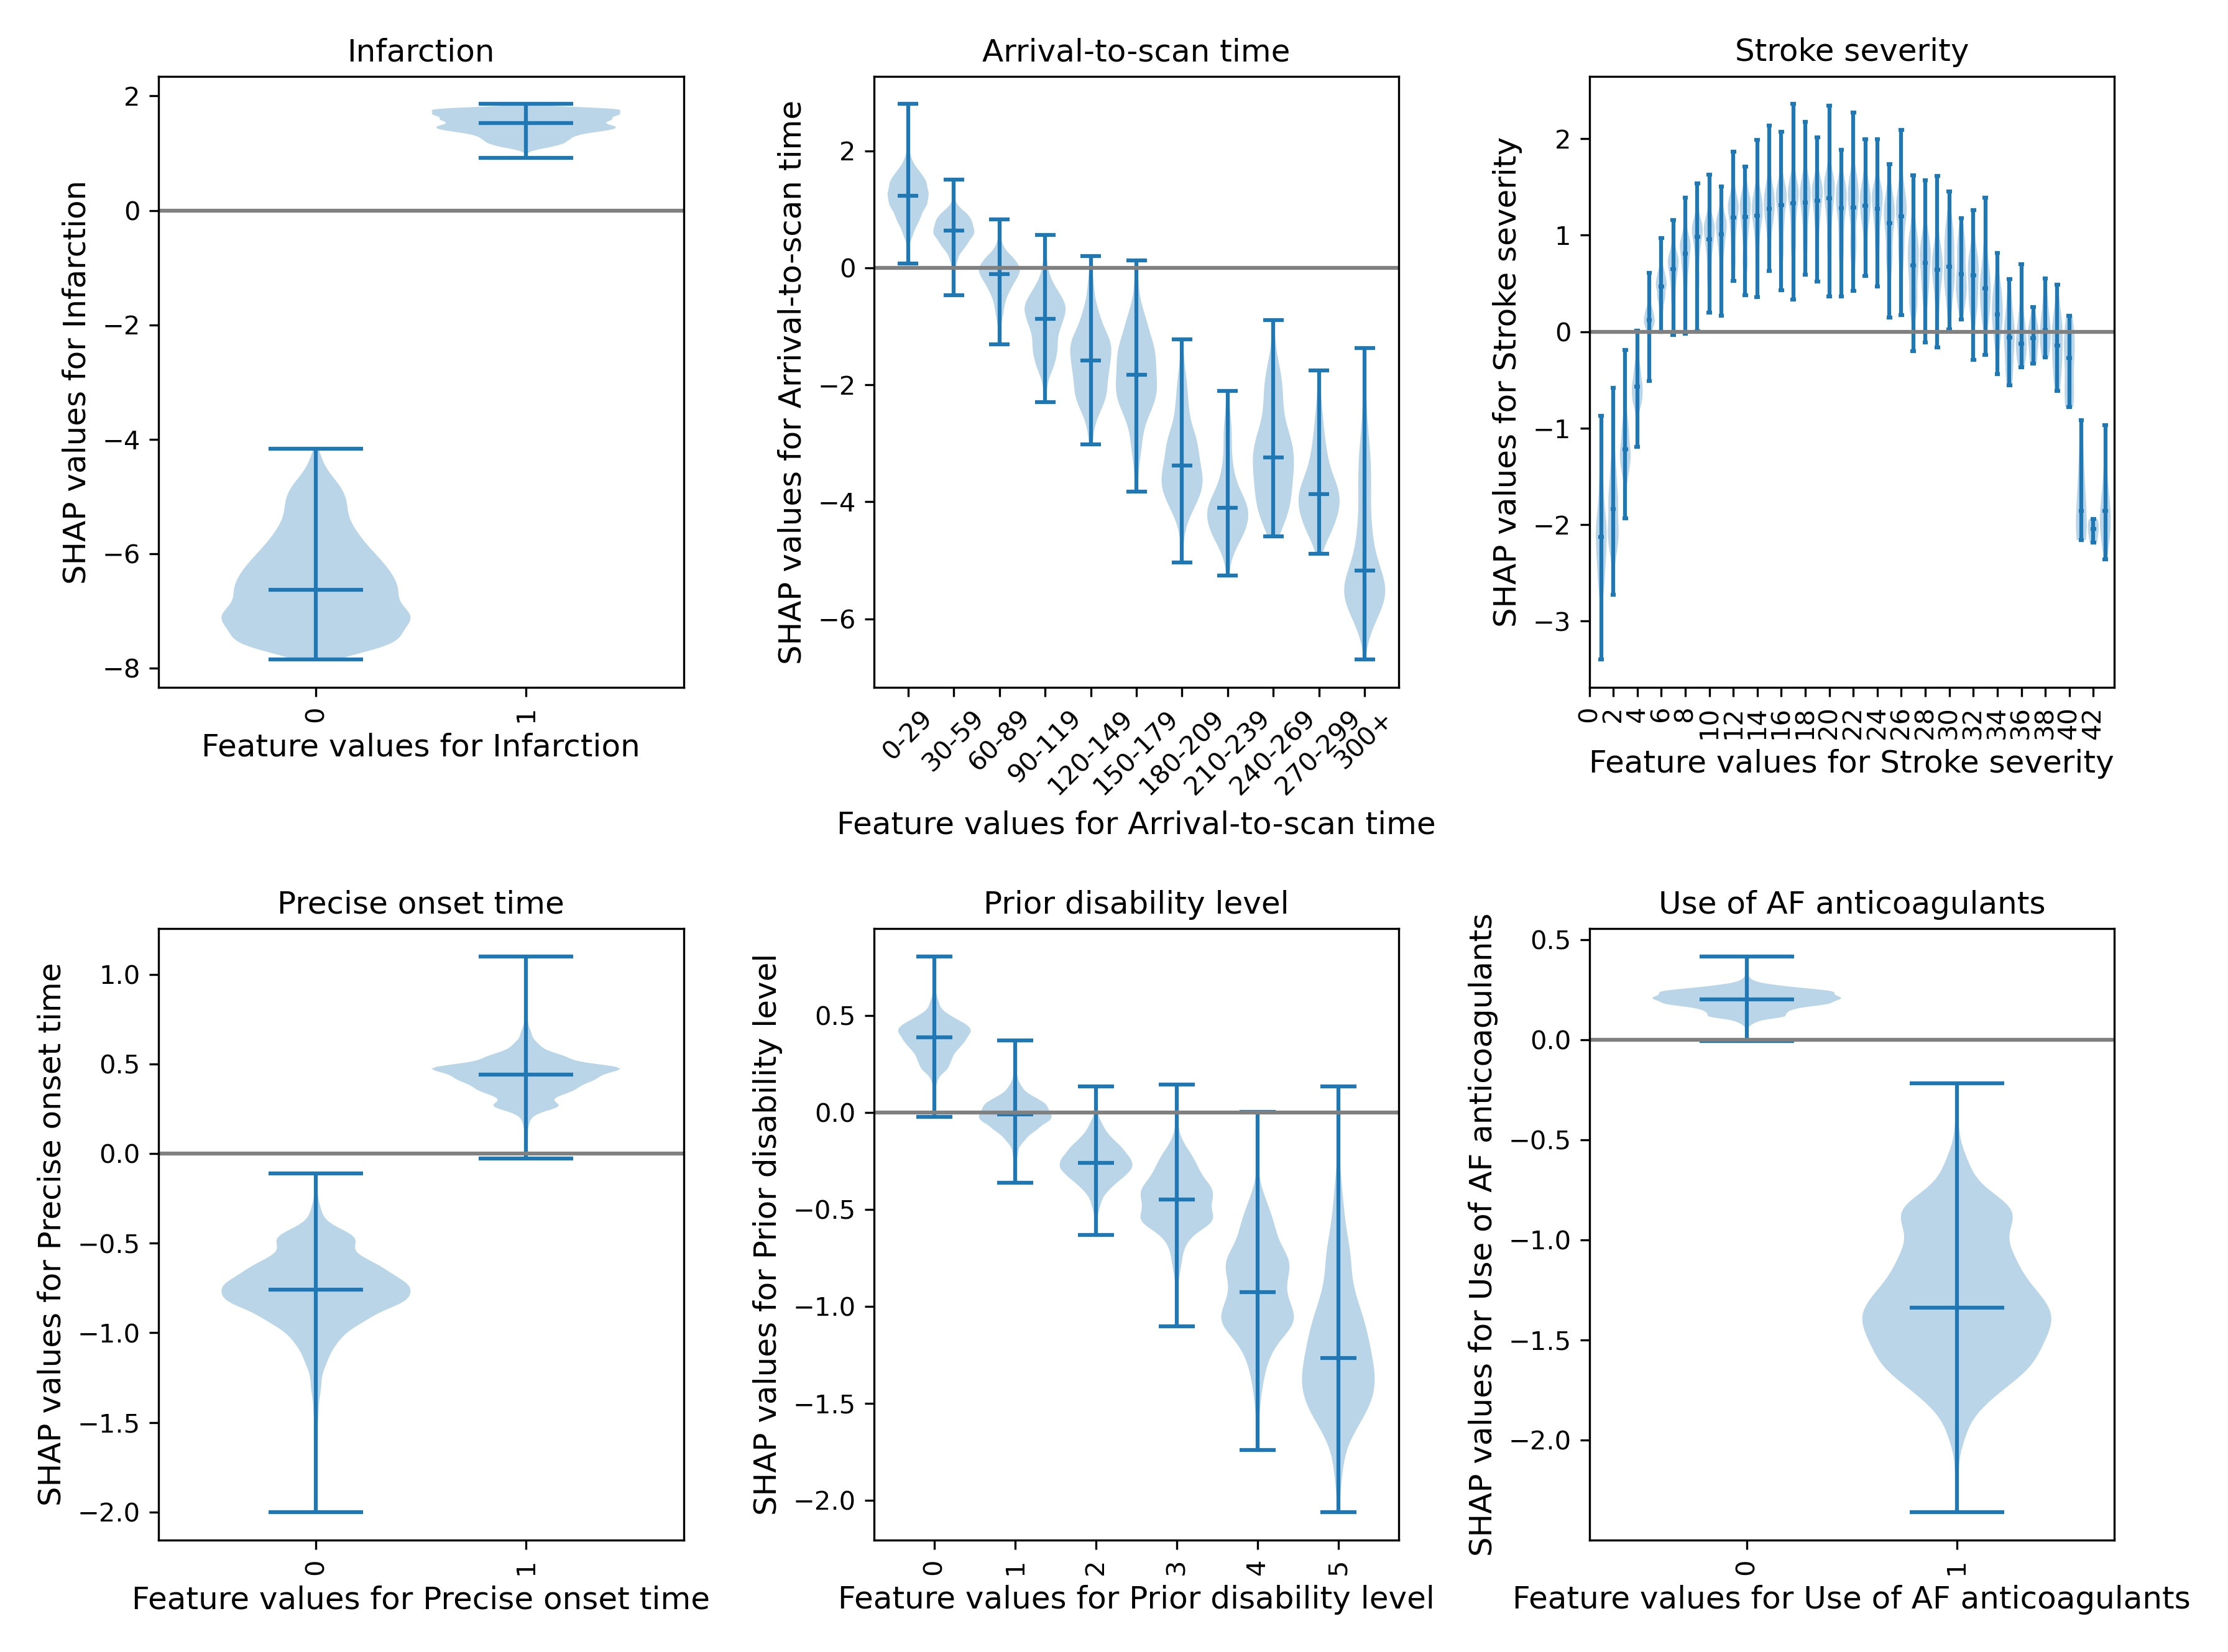
\includegraphics[width=0.80\textwidth]{./images/03_xgb_10_features_thrombolysis_shap_violin.jpg}
\end{center}
\end{frame}

%%%%%%%%%%%%%%%%%%%%%%%%%%%%%%%%%%%%%%%%%%%%%%%%%%%%%%%%%%%%%%%

\begin{frame}
\frametitle{How general effects may be modified by individual hospitals}

\begin{center}
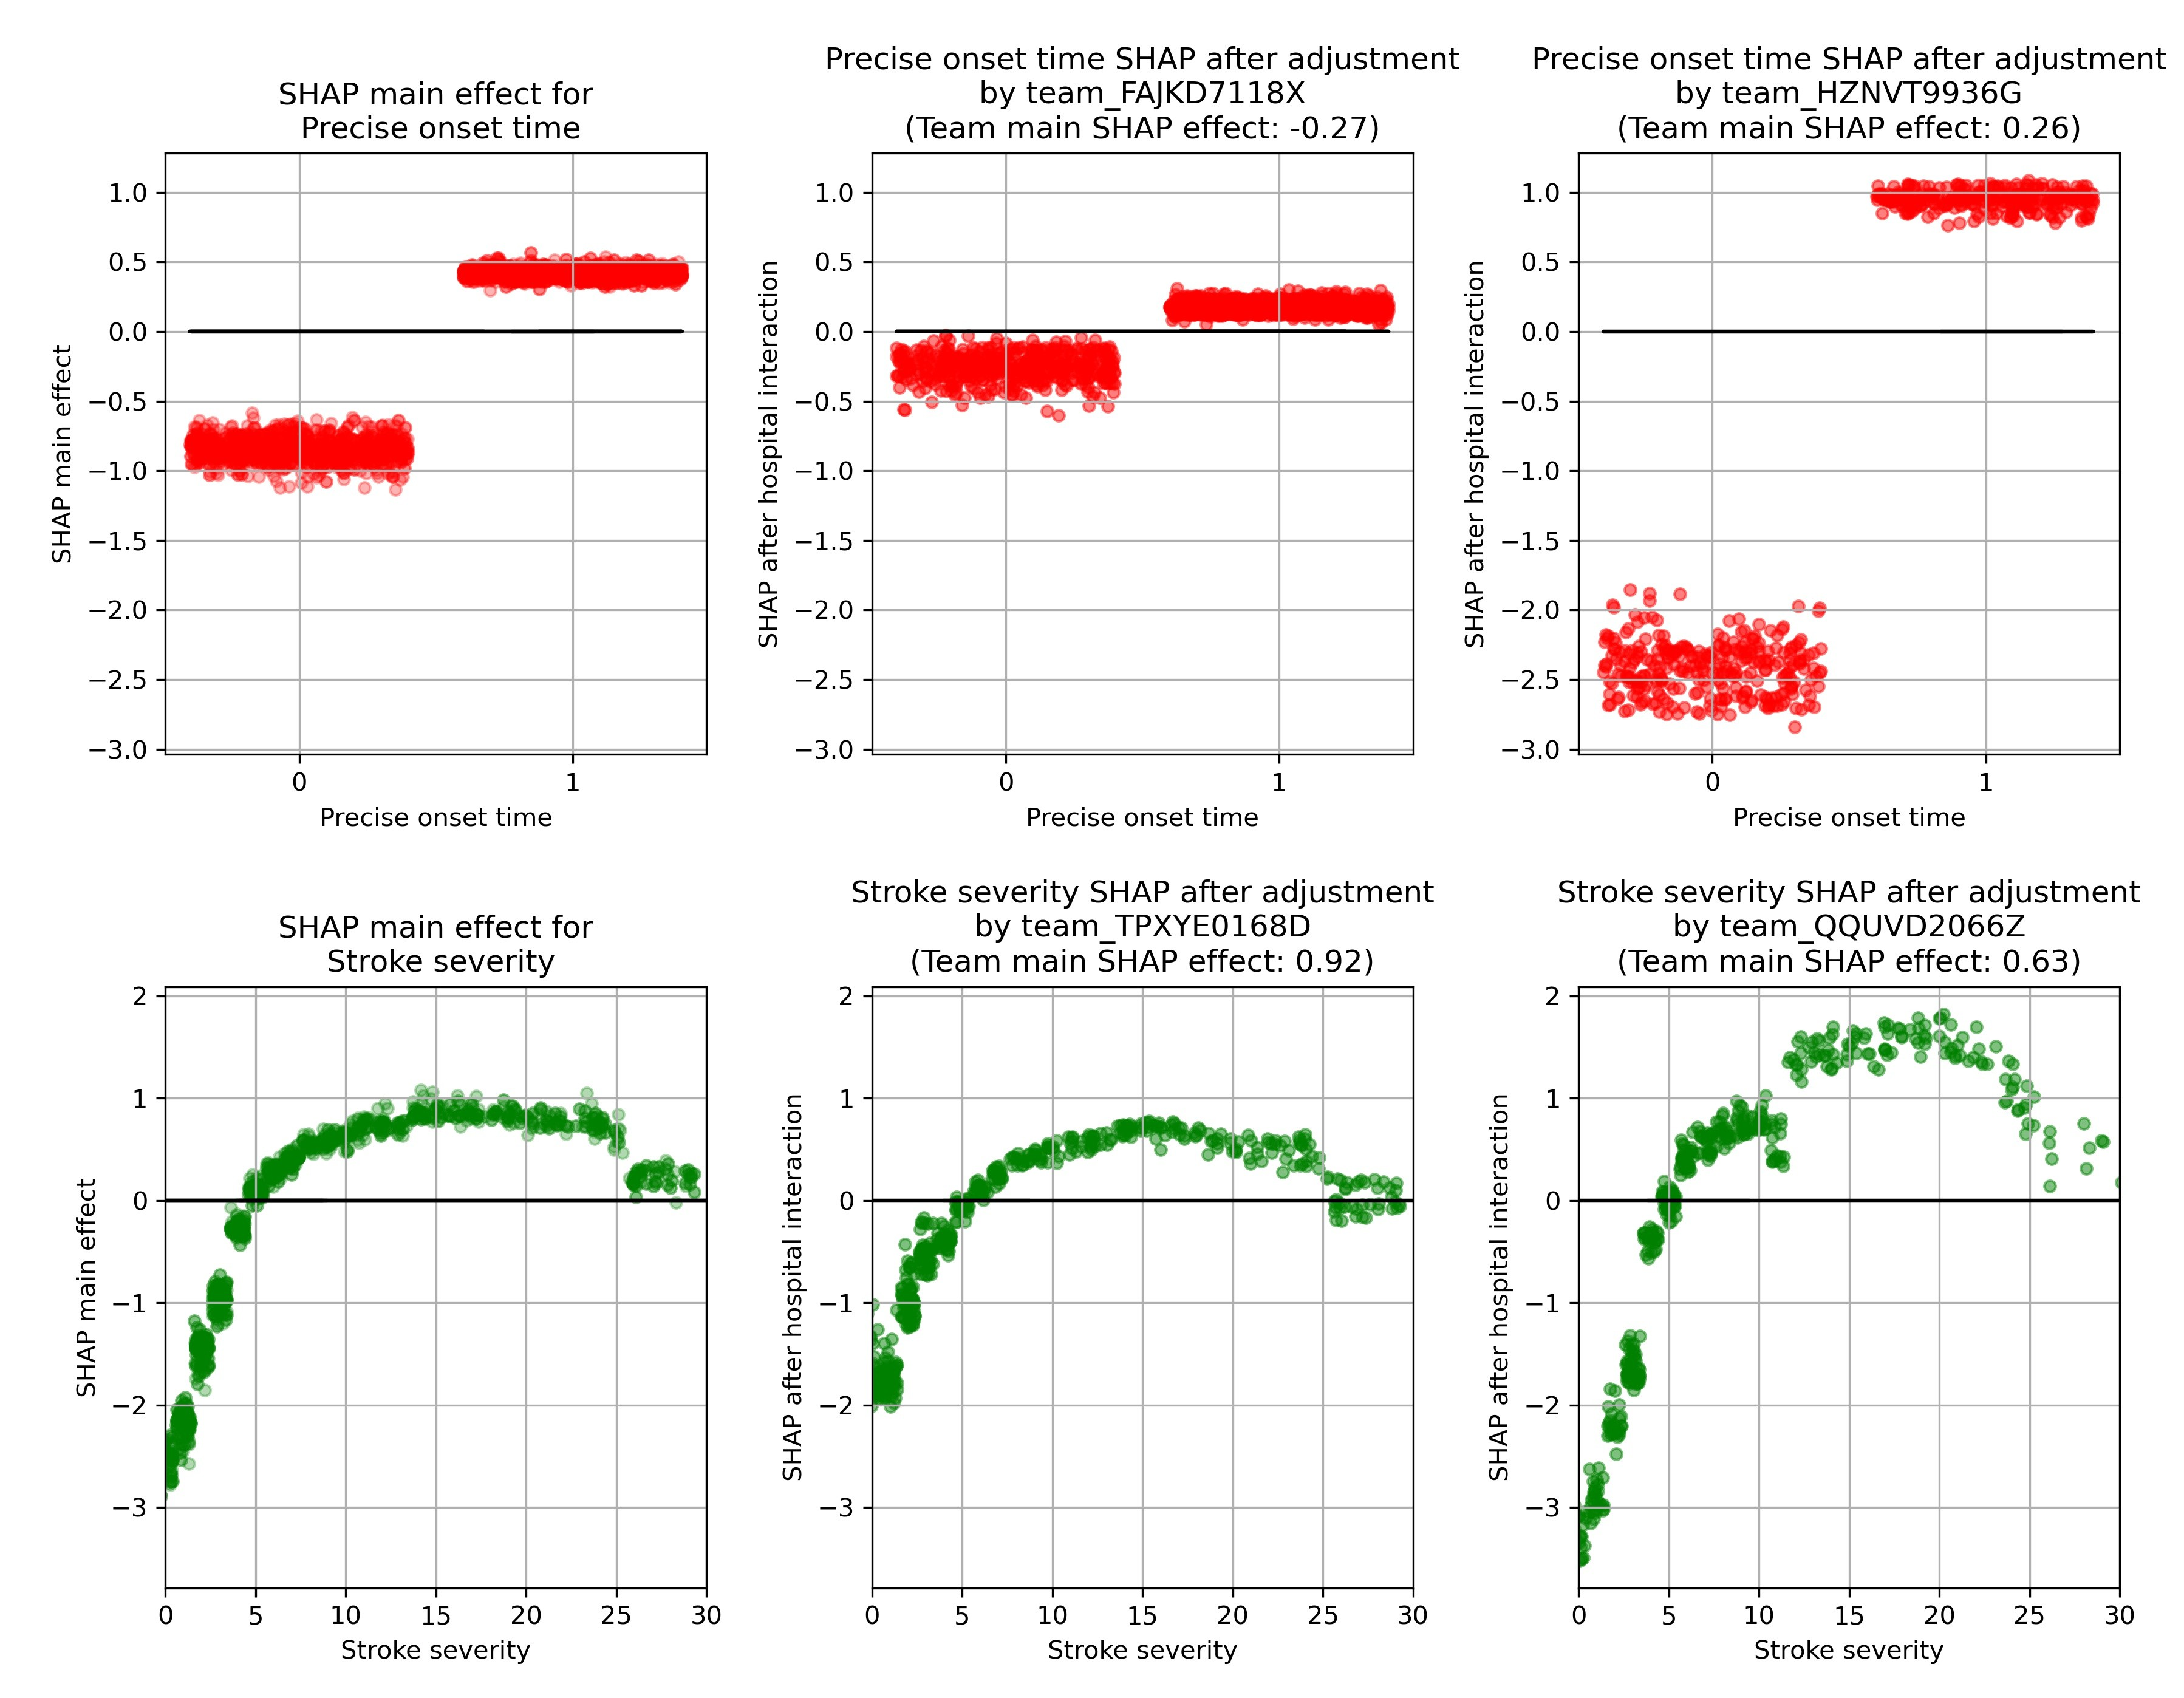
\includegraphics[width=0.80\textwidth]{./images/12aa_two_way_shap_adjustment.jpg}
\end{center}
\end{frame}

%%%%%%%%%%%%%%%%%%%%%%%%%%%%%%%%%%%%%%%%%%%%%%%%%%%%%%%%%%%%%%%

\begin{frame}
\frametitle{Thrombolysis in subgroups of patients}

\begin{center}
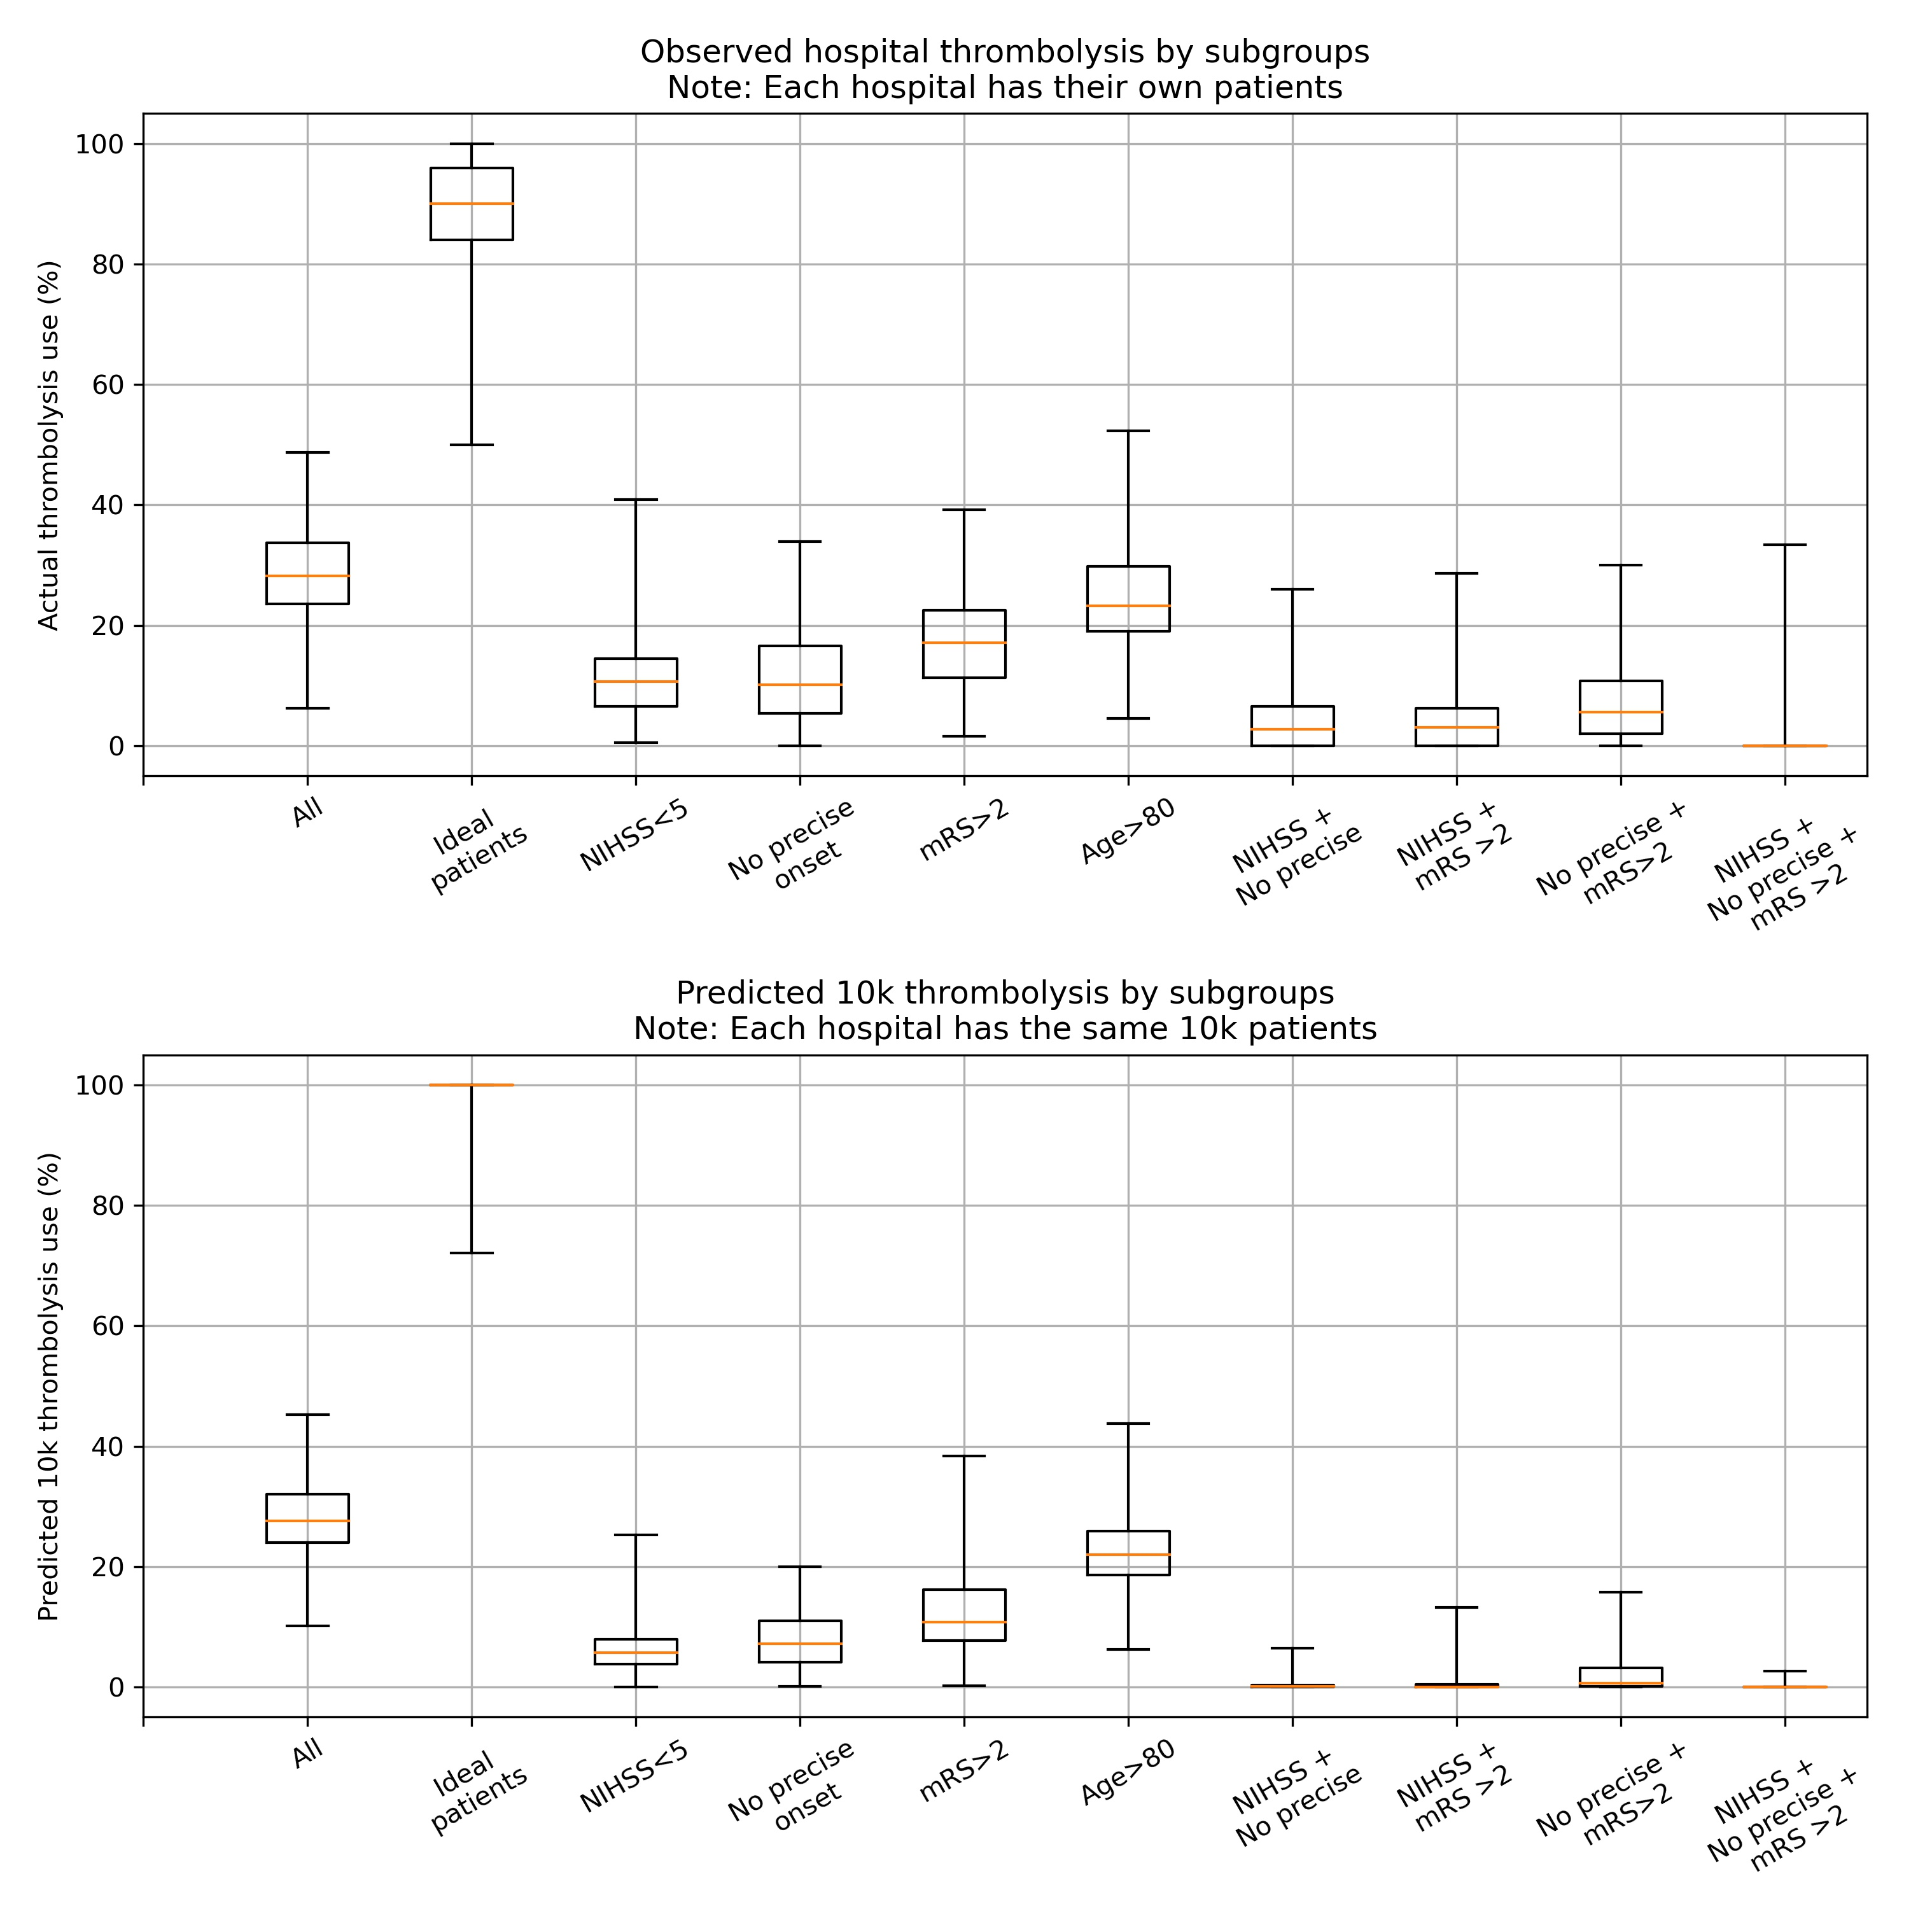
\includegraphics[width=0.69\textwidth]{./images/15a_actual_vs_modelled_subgroup_violin.jpg}
\end{center}
\end{frame}

%%%%%%%%%%%%%%%%%%%%%%%%%%%%%%%%%%%%%%%%%%%%%%%%%%%%%%%%%%%%%%%

\begin{frame}
\frametitle{How would different tems response to the same patient?}

\begin{columns}% [T] % [T] Top aligns columns

    \begin{column}{0.45\textwidth}

        \begin{footnotesize}
    
        This patient has the characteristics of a patient well-suited to thrombolysis, except they have a mild stroke.

        \vspace{3mm}
        

        \begin{itemize}
            \item Onset-to-arrival = 80 mins
            \item Arrival-to-scan = 20 mins
            \item Infarction = Yes
            \item Pre-stroke disability = 0
            \item Stroke severity (NIHSS) = 5
            \item Precise onset time = Yes
            \item Use of AF anticoagulants = No
            \item Onset during sleep = No
            \item Age = 73
        \end{itemize}
        \end{footnotesize}
        
    \end{column}
    
    \begin{column}{0.55\textwidth}
        \begin{center}
        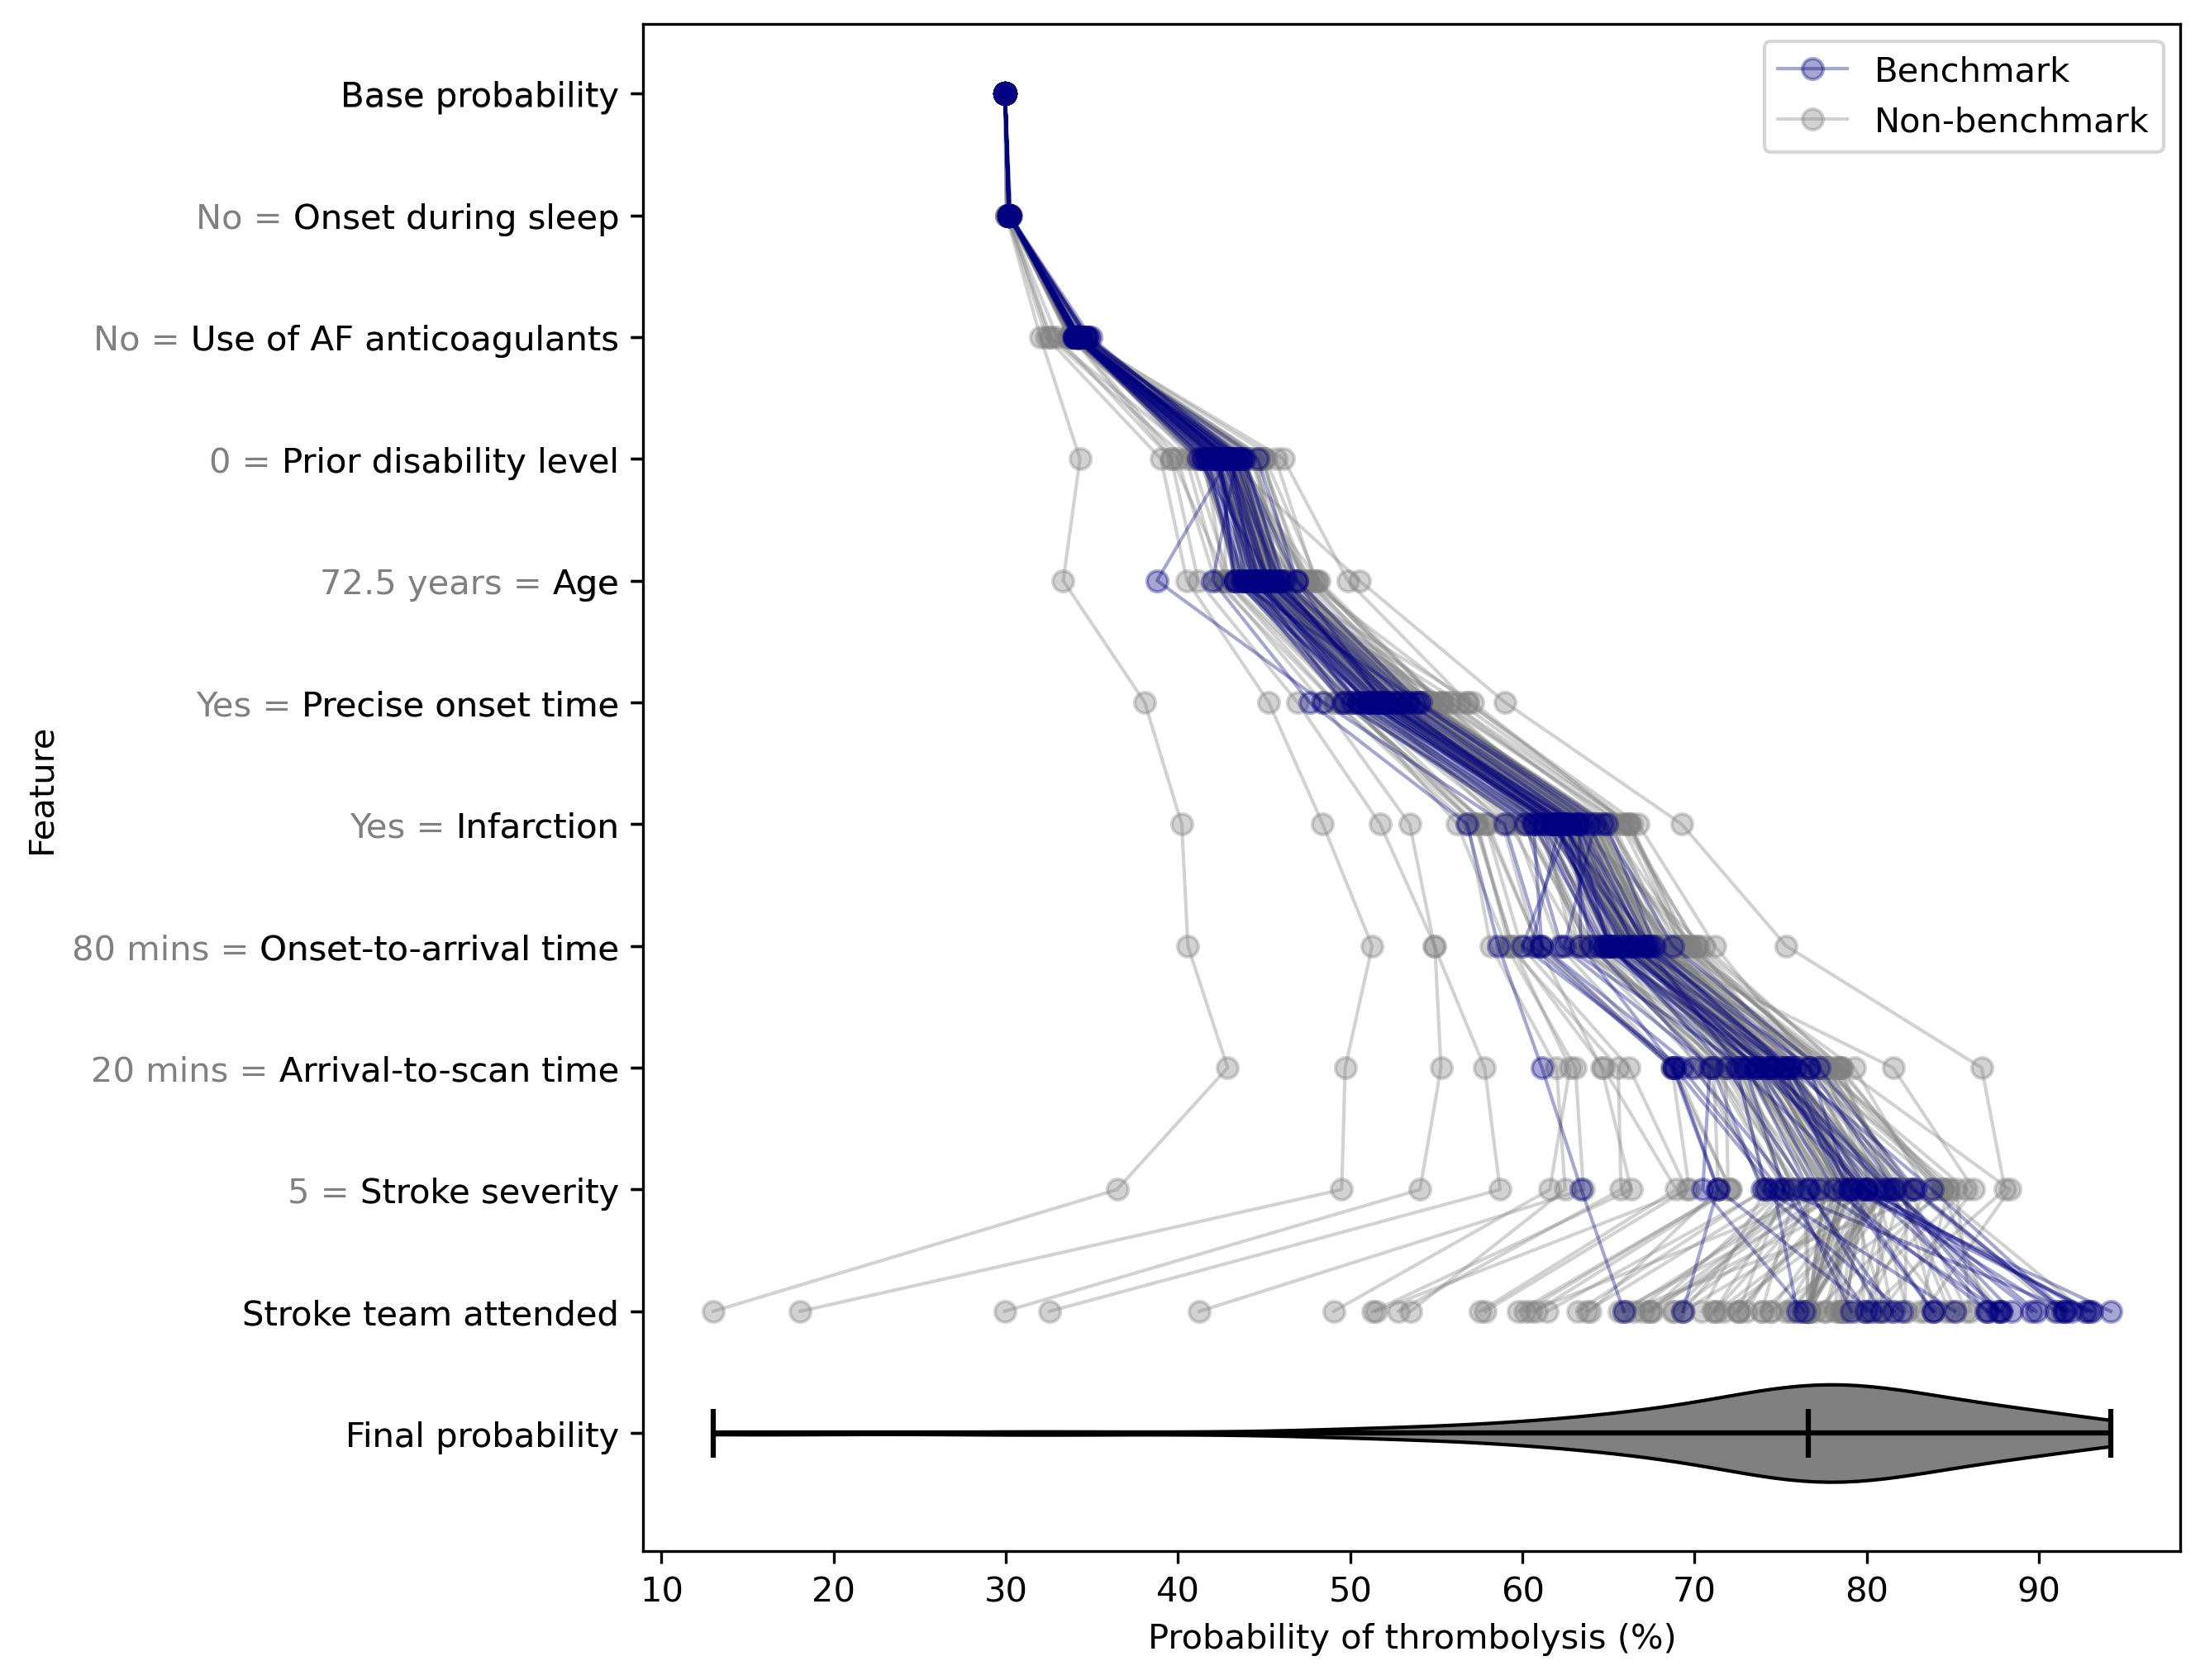
\includegraphics[width=1.0\textwidth]{./images/shap_waterfall_with_violin.jpg}
        \end{center}
    \end{column}
    
\end{columns}

\end{frame}
\end{document}




